\subsection{Databases}

\emph{Database}, \emph{RawDatabase}, \emph{RegularDatabase} and
\emph{UserDatabase} are all related to an SQL database. We would like to
add a database based on the JSON format. We need to rename the
previously cited class to show their real use (and move them into a
separate package).

\begin{itemize}
    \item \emph{Database} -> \emph{SQLDatabase}
    \item \emph{RawDatabase} -> \emph{RawSQLDatabase}
    \item \emph{RegularDatabase} -> \emph{RegularSQLDatabase}
    \item \emph{UserDatabase} -> \emph{UserSQLDatabase}
\end{itemize}

Then, we need to create interfaces which will be implemented by the databases we
need (e.g. \emph{SQLRawDatabase} implements the \emph{RawDatabase} interface).\\

Finally, we must be able to switch the type of database by modifying a property
(\emph{dbType}) in the \emph{web\_portal.cfg} file.
The database type can be tested to decide which classes to instantiate in
\emph{DatabaseFacade}. However, each time we want to add a type of
database in the application we also need to add it in the long \emph{if..else}
of the \emph{DatabaseFacade} constructor which can be seen below.\\

\begin{lstlisting}
if (dbType.equals("SQL")) {
	userDb		= new UserSQLDatabase(properties);
	regularDb	= new RegularSQLDatabase(properties);
	rawDb		= new RawSQLDatabase(properties);
} else if (dbType.equals("JSON")) {
    ...
}
\end{lstlisting}
\

These conditions can be moved outside to avoid having a huge constructor.
An Abstract Factory pattern was used, which may be a bit overkill in this case
(but it was a real application of this pattern and I wanted to try it).\\

\begin{lstlisting}
public interface AbstractDatabaseFactory {
	public RawDatabase getRawDatabase(Properties properties);
	public RegularDatabase getRegularDatabase(Properties properties);
	public UserDatabase getUserDatabase(Properties properties);
}

public class DatabaseFactoryProducer {
	/**
	 * Get a factory based on the type of database we want to use.
	 * @param type of database
	 * @return database factory for the selected type of database
	 */
	public static AbstractDatabaseFactory getFactory(String type) {
		if (type.equals("SQL")) {
			return new SQLDatabaseFactory();
		}
		
		return null;
	}
}

public class SQLDatabaseFactory implements AbstractDatabaseFactory {
	public RawDatabase getRawDatabase(Properties properties) {
		return new RawSQLDatabase(properties);
	}

	public RegularDatabase getRegularDatabase(Properties properties) {
		return new RegularSQLDatabase(properties);
	}

	public UserDatabase getUserDatabase(Properties properties) {
		return new UserSQLDatabase(properties);
	}
}

public class DatabaseFacade {
    ...
    public DatabaseFacade(Properties properties) {
    	String dbType = properties.getProperty("dbType");
    	AbstractDatabaseFactory df = DatabaseFactoryProducer.getFactory(dbType);
    	
    	userDb    = df.getUserDatabase(properties);
    	regularDb = df.getRegularDatabase(properties);
    	rawDb     = df.getRawDatabase(properties);
    }
    ...
}
\end{lstlisting}
\

Here we only have two databases implementations, but should the number grow
quickly, a more dynamic solution would be to use reflection. However using
reflection has an impact on performances and should be used as a last resort.

\begin{figure}[h!]
    \caption{Database layer diagram (1/2)}
    \centering
    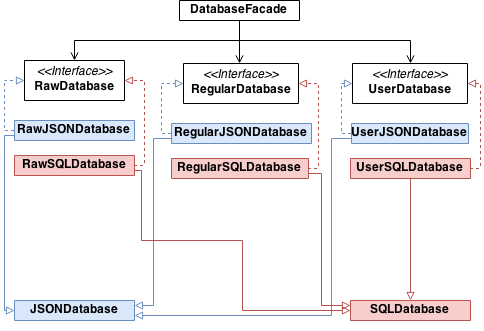
\includegraphics[width=0.6\textwidth]{images/db_diag.png}
\end{figure}

\begin{figure}[h!]
    \caption{Database layer diagram (2/2)}
    \centering
    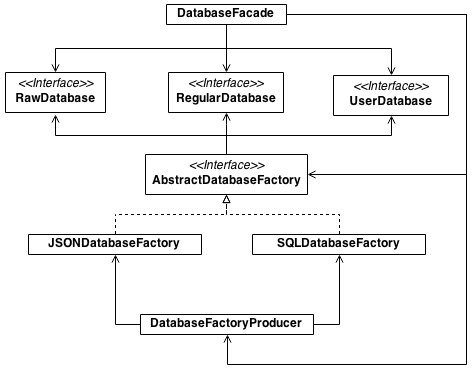
\includegraphics[width=0.6\textwidth]{images/db_fact_diag.png}
\end{figure}


\newpage
